\section{Accelerometer}

Accelerometers are used for measuring the acceleration of an object. In our case we use it to measure the acceleration of the wearable installed on a users hand and as a result of this, the users movements. When measuring the users movements, we can recognize gestures he performs.

When an object is subjected to a force, including gravity, it accelerates. Acceleration is a vector indicating a change in velocity. The acceleration can be expressed as

\begin{equation*}
a = \frac{F}{m}
\end{equation*}

where $a$ is the acceleration of the object. $F$ is the force applied to the object expresses as a vector with a force for each axis. The forces are measured in Newton. $m$ is the mass expressed as a scalar value.

In order to calculate the acceleration, the mass of the object must be known. The accelerometer determines the force applied to the object \cite[pp. 392-393]{Fraden:2112745}.

Accelerometers of varying design exist \cite[pp. 392-411]{Fraden:2112745} an example of these is the capacitive type semiconductor accelerometer which is illustrated in figure \ref{fig:accelerometer}. The accelerometer has an electrode in the middle (14) which is supported by a beam (13). The beam is flexible enough that it moves slightly up and down when the accelerometer is moved, thus moving the electrode up and down. The beam is mounted to the side of the accelerometer (2). The gap between the electrode (14) and the two stationary electrodes (25, 26) constitute two electric capacitors having capacitances of $C_1$ and $C_2$.
When the movable electrode in the middle (14) moves up and down, the capacitances $C_1$ and $C_2$ changes slightly \cite{kloeck1993capacitive}.

The changes are registered and constitutes the acceleration. This allows for measuring the acceleration on one axis. The same principle can be used to measure the acceleration on several axes.

In this project we utilize the accelerometer for recognizing gestures but other common applications of the accelerometer include pedometers, game controllers and fall detection.

\begin{figure}
\centering
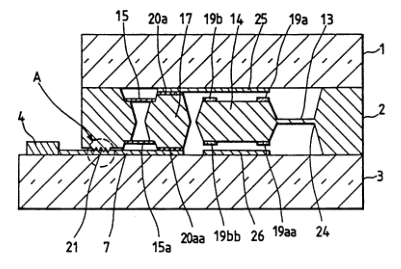
\includegraphics[width=0.5\textwidth]{images/accelerometer}
\caption{Capacitive type semiconductor accelerometer \cite{kloeck1993capacitive}.}
\label{fig:accelerometer}
\end{figure}

%%% Local Variables:
%%% mode: latex
%%% TeX-master: "../../master"
%%% End:
